\section{Performance}

As mentioned previously, the user must specify the requested cluster count \textit{k}. In order to find a suitable value for \textit{k}, the user will need to trial a number of different values. To minimize any negative effect on user-experience, therefore, it is important the clustering performs in near real-time, irrespective of terrain size and cluster count.\\

The performance of the CPU and GPU clustering implementations are analysed below along with an evaluation of the GPU speed-up. In order to evaluate the performance of the different implementations, the clustering time is analysed in relation to terrain size and cluster count. In order to accurately compare their performance, the same terrains are used with identical resources specified. All tests were performed on a machine with specifications outlined in appendix \ref{AppendixD}.

\subsection{CPU Performance}

Figure \ref{fig:cpu_clustering_performance} shows the clustering time achieved on the CPU for different terrain sizes and number of clusters. From this data, it is possible to conclude that:
\begin{itemize}
\item The clustering time increases linearly with the number of clusters to produce.
\item The clustering time is proportional to terrain area.
\end{itemize}

\begin{figure}
\center
	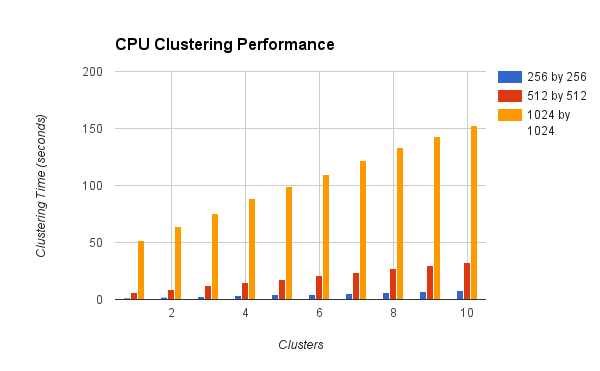
\includegraphics[width=\textwidth]{clustering_cpu_performance.png}
	\caption{ Time it takes for the clustering process to complete on the CPU depending on the cluster count. The analysis was performed for terrains of size: 256 by 256 (blue), 512 by 512 (red) and 1024 by 1024 (orange).}	
	\label{fig:cpu_clustering_performance}
\end{figure}

Although the clustering time is reasonable for smaller terrains, this processing time increases sharply with the terrain size. This is especially true when combined with an increase in the number of clusters to generate. 

\subsection{GPU Performance}

Figure \ref{fig:gpu_clustering_performance} illustrates the performance of the same tests run on the GPU. The following conclusions can be made from this data::
\begin{itemize}
\item The processing time increases linearly with cluster count but at a significantly slower rate than on the CPU. This is because individual clusters are managed in parallel on the GPU.
\item Similarly to the CPU implementation, the processing time increases linearly with terrain area. Unlike the cluster count, however, the rate of increase is comparable to that of CPU implementation. The reason for this is because, although individual terrain vertices are managed in parallel on the GPU implementation, the number of vertices far outweigh the number of GPU cores. 
\end{itemize}

\begin{figure}
\center
	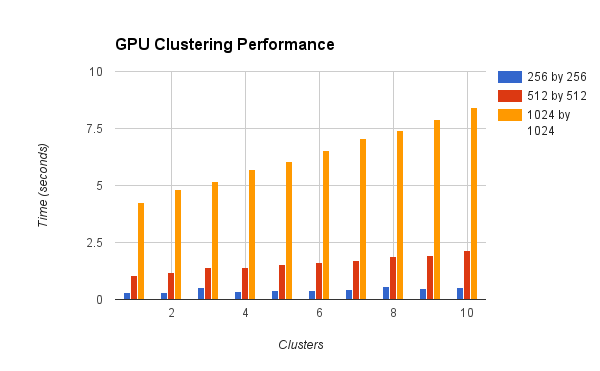
\includegraphics[width=\textwidth]{clustering_gpu_performance.png}
	\caption{ Time it takes for the clustering process to complete on the GPU depending on the cluster count. The analysis was performed for terrains of size: 256 by 256 (blue), 512 by 512 (red) and 1024 by 1024 (orange).}	
	\label{fig:gpu_clustering_performance}
\end{figure}

\subsection{GPU Speed-up}

Figures \ref{fig:clustering_cpu_v_gpu_256}, \ref{fig:clustering_cpu_v_gpu_512} and \ref{fig:clustering_cpu_v_gpu_1024} compare the CPU and GPU clustering processing time for square terrains of size 256, 512 and 1024 respectively. These histograms show that the GPU greatly outperforms the CPU, irrespective of terrain size and cluster count. Also visible in these graphics is the increased sensitivity to the cluster count of the CPU implementation over the GPU one. \\

\begin{figure}
\center
	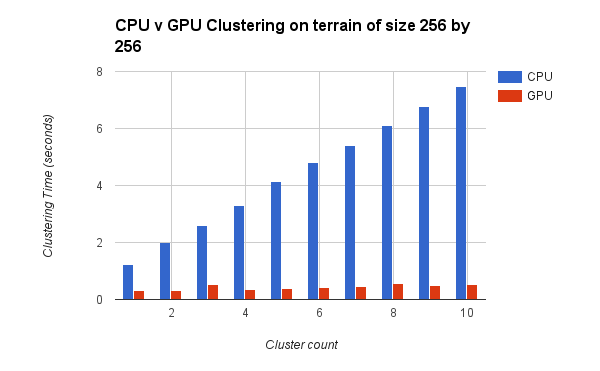
\includegraphics[width=\textwidth]{clustering_cpu_v_gpu_256.png}
	\caption{ Comparison of CPU (blue) and GPU (red) clustering times on a 256 by 256 terrain.}	
	\label{fig:clustering_cpu_v_gpu_256}
\end{figure}

\begin{figure}
\center
	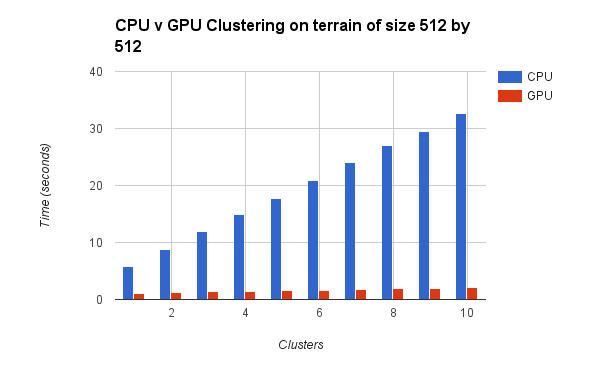
\includegraphics[width=\textwidth]{clustering_cpu_v_gpu_512.png}
	\caption{ Comparison of CPU (blue) and GPU (red) clustering times on a 512 by 512 terrain.}	
	\label{fig:clustering_cpu_v_gpu_512}
\end{figure}

\begin{figure}
\center
	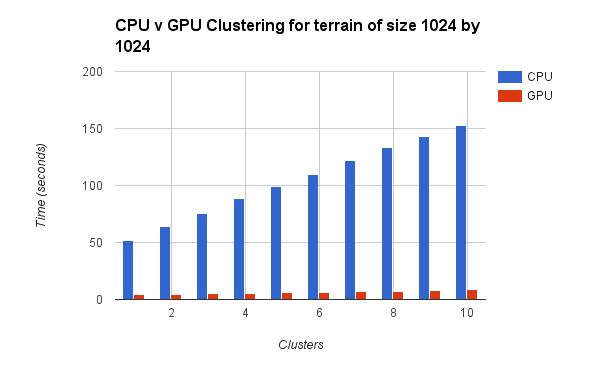
\includegraphics[width=\textwidth]{clustering_cpu_v_gpu_1024.png}
	\caption{ Comparison of CPU (blue) and GPU (red) clustering times on a 1024 by 1024 terrain.}	
	\label{fig:clustering_cpu_v_gpu_1024}
\end{figure}

As well as confirming the increased sensitivity to cluster count of the CPU implementation, figure \ref{fig:clustering_cpu_v_gpu_speedup} which plots the GPU speed-up for each terrain size and cluster count, shows the speed-up also increases with terrain size. 

\begin{figure}
\center
	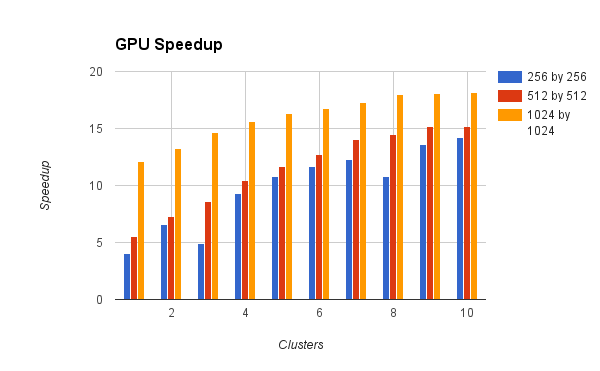
\includegraphics[width=\textwidth]{clustering_cpu_v_gpu_speedup.png}
	\caption{ Calculated clustering speed-up of the GPU implementation compared to the CPU implementation for square terrains of size 256 (blue), 512 (red) and 1024 (yellow).}	
	\label{fig:clustering_cpu_v_gpu_speedup}
\end{figure}